\documentclass[a4paper,12pt]{book}

\usepackage{lmodern}
\usepackage[utf8]{vietnam}
\usepackage{geometry}
\geometry{top=2.5cm, bottom=2.5cm, left=3cm, right=3cm}
\usepackage{titlesec}
\usepackage{setspace}

% Định dạng tiêu đề chương
\titleformat{\chapter}[display]
  {\normalfont\Large\bfseries}{\centering Tuần 1}{10pt}{\centering\Huge\bfseries}
  
\begin{document}

\chapter{Mở đầu về giải tích}


\begin{itemize}
    \item Giải tích là toán học của sự thay đổi.

    \item (lịch sử)

    \item (lịch sử)

    \item (lịch sử)
    \item (lịch sử)

\end{itemize}
\noindent Trong tuần 1, chúng tôi trình bày nội dung về hàm số và giới hạn của hàm số, đạo hàm cùng ứng dụng của chúng.
\newpage
\section{Mở đầu về giải tích}
\subsection{Đạo hàm}
Tiếp theo ta sẽ làm quen với lý thuyết về đạo hàm.
\begin{definition}
\textbf{Đạo hàm} của hàm số $f$ tại giá trị $a$, kí hiệu bởi $f'(a)$, là
    \begin{equation}
        f'(a)=\lim_{\Delta x\rightarrow 0}\frac{f(a+\Delta x)-f(a)}{\Delta x}
    \end{equation}
nếu giới hạn này tồn tại.
\end{definition}

Một trong những ý nghĩa của đạo hàm là nó thể hiện độ dốc của đồ thị và tốc độ biến thiên của hàm số, như ta có thể thấy trong hình vẽ dưới đây:

\begin{figure}[H]
\centering
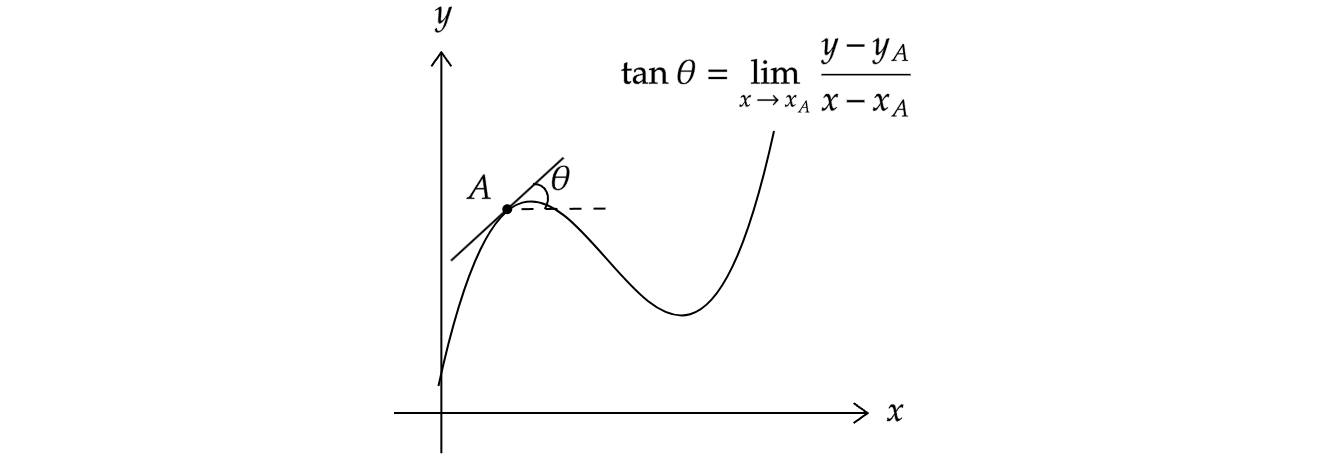
\includegraphics[width=1\textwidth]{Tuan1/ảnh/tocdobienthien.png}
\caption{Liên hệ giữa đạo hàm và độ dốc (độ lớn góc $\theta$) của đồ thị}
\end{figure}
Một ví dụ Vật Lý có thể kể đến là chuyển động của một vật. Nếu ta xét hàm số $s(t)$ là quãng đường vật đi được theo thời gian $t$, thì đạo hàm của nó tại thời điểm $t$ chính là vận tốc của vật tại thời điểm đó, kí hiệu là $v(t)=s'(t)$.

Cũng từ hình vẽ trên, ta có thể thấy đạo hàm chính là hệ số góc của tiếp tuyến đồ thị. Vì thế, ta có thể biểu diễn phương trình của đường tiếp tuyến tại $x=a$:
\begin{equation}
    y=f(a)+f'(a)(x-a)
\end{equation}
Dưới đây là đạo hàm của một số hàm thông dung:

\begin{itemize}
\item\textit{Đạo hàm của hàm đa thức}:
\begin{equation}
    \frac{d}{dx}x^n=nx^{n-1}
\end{equation}
\item\textit{Đạo hàm của các hàm lượng giác}:
\begin{center}
\begin{tabular}{cc}
\(
\begin{aligned}
    &\dfrac{d}{dx}(\sin x)=\cos x\\
    &\dfrac{d}{dx}(\cos x)=-\sin x
\end{aligned}
\)
&
\(
\begin{aligned}
    &\dfrac{d}{dx}(\tan x)=\sec^2 x\\
    &\dfrac{d}{dx}(\cot x)=-\csc^2 x
\end{aligned}
\)
\end{tabular}
\end{center}
\item\textit{Đạo hàm của hàm mũ và hàm logarit}:
\begin{equation}
    \frac{d}{dx}e^x=e^x,\quad \frac{d}{dx}\ln x=\frac{1}{x}
\end{equation}
\end{itemize}

Tương tự như giới hạn, đạo hàm cũng có một số tính chất quan trọng:
\begin{itemize}
    \item \textit{Tính chất tuyến tính}: Nếu $f(x)$ và $g(x)$ là hai hàm số theo $x$, và $c$ là một hằng số, thì
    \begin{equation}
        (cf+g)'=cf'+g'
    \end{equation}
    \item \textit{Quy tắc nhân}: Nếu $f(x)$ và $g(x)$ là hai hàm số theo $x$, thì
    \begin{equation}
        (fg)'=fg'+f'g
    \end{equation}
    \item \textit{Quy tắc chia}: Nếu $f(x)$ và $g(x)$ là hai hàm số theo $x$, với $g(x)\neq 0$, thì
    \begin{equation}
        \left(\frac{f}{g}\right)'=\frac{f'g-fg'}{g^2}
    \end{equation}
\end{itemize}

Tiếp theo ta sẽ nói về một ứng dụng quan trọng khác của đạo hàm. Nếu phóng to đồ thị tại điểm $x=a$, ta có thể thấy đồ thị hàm số trông khá giống với tiếp tuyến của nó tại điểm này.
\begin{figure}[H]
\centering
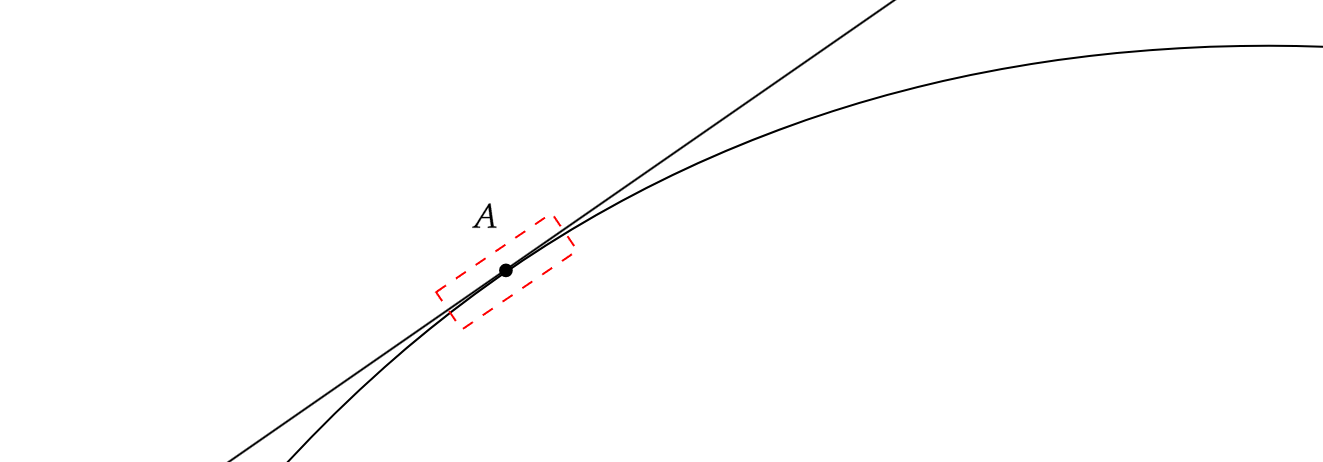
\includegraphics[width=1\textwidth]{Tuan1/ảnh/xapxituyentinh.png}
\caption{Phóng to đồ thị hàm số tại điểm $x=a$}
\end{figure}
Từ quan sát trên, ta có thể nghĩ tới một phép xấp xỉ.

\begin{definition}
    Ở lân cận điểm $x=a$, ta có thể xấp xỉ hàm số $f(x)$ bằng phương trình đường tiếp tuyến tại điểm này:
\begin{equation}
        f(x)\approx f(a)+f'(a)(x-a)
    \end{equation}
đây được gọi là \textbf{xấp xỉ tuyến tính}.
\end{definition}
Ý tưởng đằng sau phép xấp xỉ tuyến tính đôi khi được phát biểu bằng \textbf{phép lấy vi phân}.

\begin{definition}
    Nếu $y=f(x)$, \textbf{vi phân} $dx$ là một biến độc lập. Lúc đó \textbf{vi phân} $dy$ được xác định theo $dx$ bởi phương trình:
\begin{equation}
    dy=f'(x)dx
\end{equation}
\end{definition}
và \textbf{phép lấy vi phân} trên có ý nghĩa hình học như hình vẽ:

\begin{figure}[H]
\centering
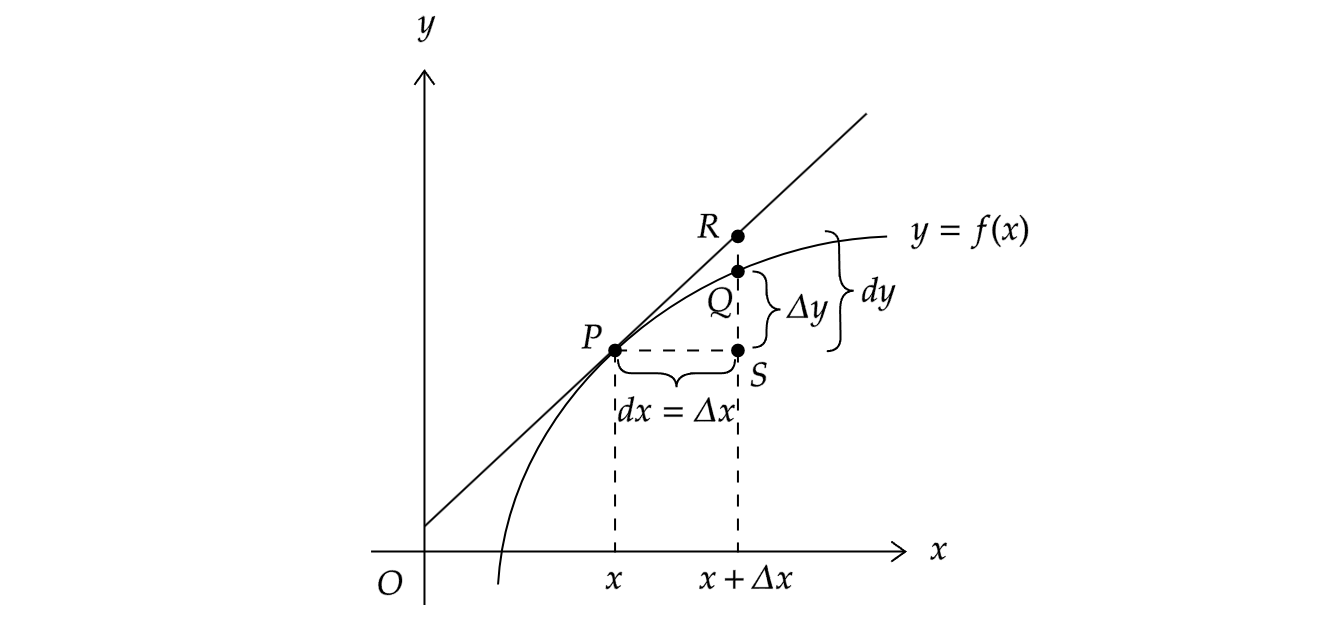
\includegraphics[width=1\textwidth]{Tuan1/ảnh/viphan.png}
\caption{Ý nghĩa hình học của phép lấy vi phân}
\end{figure}
\newpage
Nội dung của tuần được chia làm: Hàm số và Giới hạn, Đạo hàm cùng Ứng dụng của đạo hàm. Trong đó, phần Hàm số và Giới hạn đã giới thiệu khái niệm về hàm số, các cách biểu diễn hàm số (đồ thị, đại số, số liệu, lời nói) cùng với khái niệm về giới hạn hàm số đi cùng các quy tắc lấy giới hạn; phần Đạo hàm giới thiệu khái niệm về đạo hàm, ý nghĩa toán học nói chung và hình học của đạo hàm của một hàm số cùng với các quy tắc lấy đạo hàm; cuối cùng, phần Ứng dụng của đạo hàm đề cập đến các khái niệm xấp xỉ tuyến tính, vi phân, cực trị hàm số...
\vspace{5mm}
Để giúp ích cho việc làm quen kiến thức đã được trình bày và cả những kiến thức quan trọng nhưng không được trình bày, phần bài tập của tuần đã được soạn sẵn được phân chia theo một thứ tự hợp lý, khuyến khích việc làm tuần tự. Cụ thể, các bài tập được phân bố như sau:
\begin{itemize}
    \item Từ... đến ..., các phép biến đổi đồ thị hàm số: tịnh tiến và kéo giãn được giới thiệu
    \item Phần Nguyên lý quy nạp đề cập đến một phương pháp chứng minh quan trọng trong toán học, bài tập ... ứng dụng trực tiếp kiến thức về hàm số và phương pháp này. Các bài tập sau đó có sự xuất hiện của phương pháp quy nạp là ...
    \item ...
\end{itemize}
Tài liệu tham khảo kiến thức cơ bản cho tuần này là
\begin{itemize}
    \item \emph{Calculus I}, Jame Stewart, chương...
    \item ...
\end{itemize}
Ngoại trừ các tài liệu trên, bạn đọc có thể đọc thêm 
\begin{itemize}
    \item Về các ứng dụng của nguyên lý quy nạp...
    \item Về lịch sử hình thành và phát triển của giải tích..
    \item Câu chuyện về lãi suất kép và hàm $e^x$...
\end{itemize}

\end{document}
